\documentclass[11pt,aspectratio=169,xcolor={dvipsnames},hyperref={pdftex,pdfpagemode=UseNone,hidelinks,pdfdisplaydoctitle=true},usepdftitle=false]{beamer}
\usepackage{presentation}
\usepackage{tikz}

\title{Lecture 5: The New Keynesian Model Volume II}
\author{Juan Herre\~{n}o\\UCSD}
\date{2026}

% Enter presentation title to populate PDF metadata:
\newcommand{\Cov}{\text{Cov}_\lambda}
\newcommand{\El}{\mathbb{E}_\lambda}
\newcommand{\mm}{\text{{\fontfamily{qzc}\selectfont m}}}

\begin{document}

\maketitle

\begin{frame}
\frametitle{The Three Equation Model}
	\begin{align*}
		\hat{y}_t &=-\sigma[\hat{i}_t-E_t\{\hat{\pi}_{t+1}\}]+E_t\{\hat{y}_{t+1}\} \\
		\hat{\pi}_t&=\kappa (\hat{y}_t-\hat{y}_t^{n}) +\beta E_t \{\hat{\pi}_{t+1}\} \\
		\hat{i}_t&=\phi_\pi\hat{\pi}_t+v_t \\
	\end{align*}
\begin{itemize}
\item Imagine a contractionary MP shock $v_t >0$ that increases the nominal interest rate
\item Returns to saving increase, households intertemporally substitute, decreasing $\hat{c}_t$ by $\sigma$
\item Market clearing implies that $\hat{y}_t$ decreases
\item Since $\hat{y}_t$ decreases inflation by $\kappa$
\item Households form model-consistent expectations about $ \hat{\pi}_{t+1}$
\item The decrease in inflation counteracts the effects on $\hat{i}$
\item Changes in $E_t\{\hat{\pi}_{t+1}\}$ affect output
\item and on and on and on
\end{itemize}
What is an equilibrium? A point at which all equations are consistent.
\end{frame}


\begin{frame}{The New Keynesian Model in words}
\begin{itemize}
\item Interest rates go down. Households intertemporally substitute to consume more. Consumption demand needs to be satisfied, so firms need to produce more. To produce more, firms need to hire more labor. To hire more labor, firms need to pay higher wages. Higher wages increase the marginal cost of production of firms. Firms pass-through those costs to prices according to the slope of the Phillips curve, generating inflation.
\item Key parameters:
\begin{itemize}
\item How strongly households intertemporally substitute: $\sigma = 1/\gamma$
\item How much do wages have to go up to accommodate more demand (Frisch and wealth effects)? $\varphi$, $\gamma$
\item How much marginal costs push inflation $\kappa$.
\end{itemize}
\end{itemize}
\end{frame}

\begin{frame}{Today}
\begin{itemize}
\item Today we will do something very simple. We will inspect this model ``under the hood''
\item Is the NK model efficient?
\item What are its sources of inefficiency?
\item What do we lose by log-linearizing?
\item What is the shape of the IRFs implied by the model?
\item How do they correspond with those estimated in the data?
\end{itemize}
\end{frame}


\begin{frame}{Inefficient Markups in Steady State}
\begin{itemize}
\item The decentralized equilibrium is inefficient even with flexible prices
\item Intuition: Firms are too small as they try to exploit their monopoly power
\item ``too small'' means that the planner would choose larger firm sizes
\item Caution. That in this model markups are inefficient does not mean that markups are always inefficient. Large class of models with entry costs, where without markups production would not take place.
\end{itemize}
\end{frame}

\begin{frame}{Inefficient Markup in Steady State}
\begin{itemize}
\item Descentralized economy under flexible prices
\begin{align*}
1 = \frac{P_{it}}{P_t} = \frac{\theta}{\theta-1} \frac{W_t}{A_t} \frac{1}{P_t}
\end{align*} 
\item Use the labor supply curve $\frac{W_t}{P_t} = \chi N_t^{\varphi}C_t^{\gamma}$
\item And use that under flexible prices $L_t = \int_0^1 L_{it} di = \frac{Y_t}{A_t}$ to find:
\begin{align*}
Y_t = A^{\frac{\varphi+1}{\gamma + \varphi}}_t \chi^{-1/(\gamma + \varphi)} \left(\frac{\theta}{\theta-1}\right)^{-1/(\gamma + \varphi)}
\end{align*}
\item Output is decreasing in the flexible price markup
\end{itemize}
\end{frame}


\begin{frame}{Inefficient Markup in Steady State}
\begin{itemize}
\item Compare with a planner that chooses allocations directly
\item The planner will choose $C_{it} = C_{jt}$ $\forall i,j$
\item So the problem of the planner is
\begin{align*}
\max \frac{C_t^{1-\gamma}}{1-\gamma} - \chi \frac{N_t^{1+\varphi}}{1+\varphi}
\end{align*}
\item Subject to market clearing and technologies $C_t = Y_t$, and $Y_t = A_t N_t$
\item Solve that simple problem
\begin{align*}
Y_t = A^{\frac{\varphi+1}{\gamma + \varphi}}_t \chi^{-1/(\gamma + \varphi)}
\end{align*}
\item This solution guarantees that $MRS_t = MPL_t$ which given our functional forms reduces to
$$\chi N_t^{\varphi} C_t^{\gamma} = A_t$$
\end{itemize}
\end{frame}

\begin{frame}{Inefficient Markup in Steady State}
\begin{itemize}
\item Descentralized Equilibrium yields:
\begin{align*}
Y_t = A^{\frac{\varphi+1}{\gamma + \varphi}}_t \chi^{-1/(\gamma + \varphi)} \left(\frac{\theta}{\theta-1}\right)^{-1/(\gamma + \varphi)}
\end{align*}
\item And Planner's problem
\begin{align*}
Y_t = A^{\frac{\varphi+1}{\gamma + \varphi}}_t \chi^{-1/(\gamma + \varphi)}
\end{align*}
\item You can check that the decentralized equilibrium attains lower welfare. Inefficiency.
\end{itemize}
\end{frame}

\begin{frame}{Inefficient Markup in Steady State}
\begin{itemize}
\item Easy to correct if the planner has access to lump-sum transfers
\item Idea: The issue is that firms charge prices $P_{it} = \frac{\theta}{\theta-1} \frac{W_t}{A_t}$ as opposed to $P_{it} =\frac{W_t}{A_t}$
\item Imagine the planner imposes a payroll subsidy. Firms pay $W_t(1-\tau)$ for each worker. Optimal pricing yields
\begin{align*}
 P_{it} = \frac{\theta}{\theta-1} \frac{W_t(1-\tau)}{A_t}
 \end{align*}
 \item If planner chooses $\tau = 1/\theta$, then $\frac{\theta}{\theta-1} (1-\tau) = 1$, recovering efficiency
 \item Key: Access to lump-sum transfers so that households pay for the subsidy without distorting their labor supply
 \end{itemize}
\end{frame}


\begin{frame}{Inefficient Cyclical Markup}
\begin{itemize}
\item Define the aggregate markup as the ratio of aggregate prices to aggregate marginal costs
\begin{align*}
\mathcal{M}_t = \frac{P_t}{MC_t} = \frac{P_t}{(1-\tau)W_t/A_t} 
\end{align*}
\item Solve for the real wage
\begin{align*}
\frac{W_t}{P_t} = \frac{A_t}{(1-\tau) \mathcal{M}_t}
\end{align*}
\item Notice that $\frac{1}{(1-\tau)} = \frac{\theta}{\theta-1} \equiv \mathcal{M}$
\begin{align*}
\frac{W_t}{P_t} = A_t \frac{\mathcal{M}}{\mathcal{M}_t}
\end{align*}
\item Unless $\frac{\mathcal{M}}{\mathcal{M}_t} = 1$, then
\begin{align*}
MRS_t \neq MPL_t
\end{align*}
\end{itemize}
\end{frame}


\begin{frame}{Inefficient Cyclical Markup}
\begin{align*}
\frac{W_t}{P_t} = A_t \frac{\mathcal{M}}{\mathcal{M}_t}
\end{align*}
\begin{itemize}
\item Intuition. Due to price rigidity, an aggregate shock may move the average markup that firms charge
\item The aggregate markup will be either too large or too small. And consequently, there will be too little or too much production
\item Because this inefficiency is dynamic (it has a $t$ subscript), it cannot be corrected with a constant tax/subsidy
\item Can only be corrected with an instrument that keeps the aggregate markup constant at $\mathcal{M}$.
\end{itemize}
\end{frame}

\begin{frame}{Inefficient Price Dispersion}
\begin{itemize}
\item Price rigidity introduces additional inefficiencies
\item Intuition. Varieties enter symmetrically in the utility function
\item They all have the same marginal cost
\item But due to staggered price adjustment they will have different prices
\item Different goods that cost the same will have different prices
\item Inducing \textit{relative price} dispersion
\item The planner does not like that.
\end{itemize}
\end{frame}


\begin{frame}{Inefficient Price Dispersion}
\begin{itemize}
\item Aggregate labor demand
\begin{align}
L_t = \int_0^1 L_{it} di
\end{align}
\item Use the production function and the demand curve
\begin{align}
L_t = \frac{Y_t}{A_t} \int_0^1 \left(\frac{P_{it}}{P_t}\right)^{-\theta} di
\end{align}
\item Solve for $Y$
\begin{align*}
Y_t = D_t A_t L_t
\end{align*}
\item for $D_t = \left( \int_0^1 \left(\frac{P_{it}}{P_t}\right)^{-\theta} di\right)^{-1}$
\item $D$ as a productivity wedge on the aggregate production function
\end{itemize}
\end{frame}


\begin{frame}{Inefficient Price Dispersion}
\begin{itemize}
\item A second-order approximation of $\int_0^1 \left(\frac{P_{it}}{P_t}\right)^{-\theta} di$ yields:
\begin{align*}
\int_0^1 \left(\frac{P_{it}}{P_t}\right)^{-\theta} di \approx 1 + \frac{1}{2}\theta var_i(\hat{p}_{it}) > 1
\end{align*}
\item Proof: Gali appendix 3.3
\item Price dispersion reduces aggregate output (and consumption)
\item Price dispersion only shows up to the second-order
\item A log-linearized model misses this crucial channel
\item Key insight: Even though consumers do not care about prices directly, staggered price adjustment induces an inefficiency on aggregate consumption, with consequences on welfare
\end{itemize}
\end{frame}


\begin{frame}{Key Economics}
\begin{itemize}
\item Model with flexible prices:
\begin{itemize}
\item Workers are on their labor supply curve. 
$$\frac{W_t}{P_t} = \chi C_t^{\gamma} N_t^{\varphi} = MRS_t$$ always holds
\item Firms are on their labor demand curves
$$ \frac{W_t}{P_t} = A_t F'(N_t) = MPL_t$$ always holds
\item therefore $$MPL_t = MRS_t$$
\end{itemize}
\end{itemize}
\end{frame}

\begin{frame}{Key Economics}
\begin{itemize}
\item Model with sticky prices
\begin{itemize}
\item Workers are on their labor supply curve. 
$$\frac{W_t}{P_t} = \chi C_t^{\gamma} N_t^{\varphi} = MRS_t$$ always holds
\item Firms are \textbf{not} on their labor demand curves
$$ \frac{W_t}{P_t} \neq A_t F'(N_t) = MPL_t$$ does not need to hold
\item What determines labor demand then?
\item Product demand + production function
$$\hat{y}_t = \mathbb{E}_t \hat{y}_{t+1} - \sigma (i_t - \mathbb{E}_t \hat{\pi}_{t+1})$$
\item Makes clear that the central bank is key to determine market clearing in the labor market
\end{itemize}
\end{itemize}
\end{frame}


\begin{frame}{The natural rate of interest}
\begin{itemize}
\item Our Euler equation	$\hat{y}_t =-\sigma[\hat{i}_t-\mathbb{E}_t \hat{\pi}_{t+1} ]+\mathbb{E}_t \hat{y}_{t+1} $
\item We can rewrite in terms of the output gap. Subtract and add $\hat{y}^n_t$ and $\mathbb{E}_t \hat{y}^n_{t+1}$
\begin{align}
\tilde{y}_t =-\sigma[\hat{i}_t-\mathbb{E}_t \hat{\pi}_{t+1} ]+\mathbb{E}_t \tilde{y}_{t+1}  + \mathbb{E}_t \Delta \hat{y}^n_{t+1}
\end{align}
\item where $\tilde{y} = \hat{y} - \hat{y}^n$ is the output gap.
\item Or alternatively
\begin{align}
\tilde{y}_t =-\sigma[\hat{i}_t-\mathbb{E}_t \hat{\pi}_{t+1} - \hat{r}^n_t ]+\mathbb{E}_t \tilde{y}_{t+1} 
\end{align}
\item where $\hat{r}^n_t = \frac{1}{\sigma}  \mathbb{E}_t \Delta \hat{y}^n_{t+1}$ is the real interest rate that prevails in the flexible price equilibrium
\item Clarifies that $\tilde{y}$ reacts to the gap in real interest rates wrt flexible price eq.\item The natural rate of interest will be important when we think of optimal policy design
\item Intuitively, if the central bank can keep a real rate consistent with the natural rate, then the output gap will be zero
\end{itemize}
\end{frame}



\begin{frame}{Length of Monetary Policy Effects}
\begin{itemize}
\item Tempting to think the following:
\begin{quote}
If 10\% of firms adjust their prices every month, then after 10 months every firm will have adjusted their prices, and the economy will behave as if money was neutral starting in month 11, so the effects of monetary shocks will vanish pretty soon
\end{quote}
\item I get migraines whenever I hear that. Two issues:
\begin{itemize}
\item (1): In the Calvo model price adjustment is random, so after 10 months, 35\% of firms have yet to adjust. Many price adjustments will be ``wasted'' on firms that have adjusted already.
\item (2): The argument assumes that adjusters will change their price to flexible price counterpart when given the chance. But that may not be the case if:
\begin{itemize}
\item Firms do not want to separate too much from their competitors to not lose demand
\item Nominal frictions make it so that marginal costs (think wages) do not move much
\end{itemize}
\item These reasons are called in the literature ``real rigidities'' and we will talk about them extensively.
\item In terms of math. There is a difference between the effect of price rigidity $\alpha$, and $\kappa$. $\kappa$ and $\alpha$ may be substantially different
\end{itemize}
\end{itemize}
\end{frame}

\begin{frame}{The New Keynesian Phillips Curve is front-loaded}
\begin{itemize}
\item Inflation is the PV of future expected output gaps $\times$ the slope of the Phillips curve
\begin{align}
\hat{\pi}_t = \kappa \mathbb{E}_t \sum_{k=0}^{\infty} \beta^k (\hat{y}_{t+k} - \hat{y}^n_{t+k})
\end{align}
\item News of a sequence of $ (\hat{y}_{t+k} - \hat{y}^n_{t+k}) <0$ . Inflation reaches a trough at period $t$

\tikzset{every picture/.style={line width=0.75pt}} %set default line width to 0.75pt        
\begin{figure}
\centering
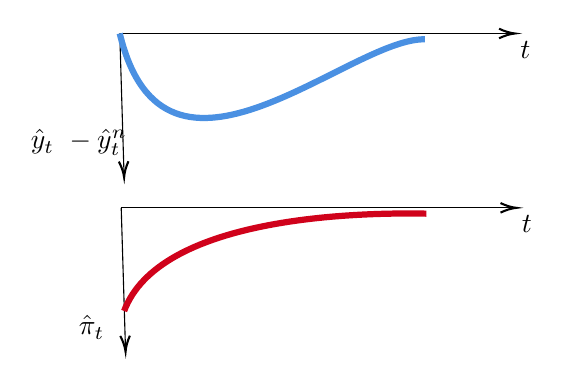
\begin{tikzpicture}[x=0.75pt,y=0.75pt,yscale=-1,xscale=1,scale = 0.7]
%uncomment if require: \path (0,243); %set diagram left start at 0, and has height of 243

%Straight Lines [id:da323586868742042] 
\draw    (212,13) -- (214.94,110) ;
\draw [shift={(215,112)}, rotate = 268.26] [color={rgb, 255:red, 0; green, 0; blue, 0 }  ][line width=0.75]    (10.93,-3.29) .. controls (6.95,-1.4) and (3.31,-0.3) .. (0,0) .. controls (3.31,0.3) and (6.95,1.4) .. (10.93,3.29)   ;
%Straight Lines [id:da82357276970792] 
\draw    (212,13) -- (482,13) ;
\draw [shift={(484,13)}, rotate = 180] [color={rgb, 255:red, 0; green, 0; blue, 0 }  ][line width=0.75]    (10.93,-3.29) .. controls (6.95,-1.4) and (3.31,-0.3) .. (0,0) .. controls (3.31,0.3) and (6.95,1.4) .. (10.93,3.29)   ;
%Curve Lines [id:da5275876554887928] 
\draw [color={rgb, 255:red, 74; green, 144; blue, 226 }  ,draw opacity=1 ][line width=2.25]    (212,13) .. controls (243,142) and (370,16) .. (422,17) ;

%Straight Lines [id:da14528408933465897] 
\draw    (213,133) -- (215.94,230) ;
\draw [shift={(216,232)}, rotate = 268.26] [color={rgb, 255:red, 0; green, 0; blue, 0 }  ][line width=0.75]    (10.93,-3.29) .. controls (6.95,-1.4) and (3.31,-0.3) .. (0,0) .. controls (3.31,0.3) and (6.95,1.4) .. (10.93,3.29)   ;
%Straight Lines [id:da2165312985641039] 
\draw    (213,133) -- (483,133) ;
\draw [shift={(485,133)}, rotate = 180] [color={rgb, 255:red, 0; green, 0; blue, 0 }  ][line width=0.75]    (10.93,-3.29) .. controls (6.95,-1.4) and (3.31,-0.3) .. (0,0) .. controls (3.31,0.3) and (6.95,1.4) .. (10.93,3.29)   ;
%Curve Lines [id:da3052536679804041] 
\draw [color={rgb, 255:red, 208; green, 2; blue, 27 }  ,draw opacity=1 ][line width=2.25]    (215,204) .. controls (239,140) and (371,136) .. (423,137) ;

% Text Node
\draw (486,16.4) node [anchor=north west][inner sep=0.75pt]    {$t$};
% Text Node
\draw (149,77.4) node [anchor=north west][inner sep=0.75pt]    {$\hat{y}_{t} \ -\hat{y}_{t}^{n} \ $};
% Text Node
\draw (487,136.4) node [anchor=north west][inner sep=0.75pt]    {$t$};
% Text Node
\draw (182,205.4) node [anchor=north west][inner sep=0.75pt]    {$\hat{\pi }_{t} \ $};
\end{tikzpicture}
\end{figure}
\end{itemize}
\end{frame}

\begin{frame}{NK Model is too forward looking}
\begin{figure}
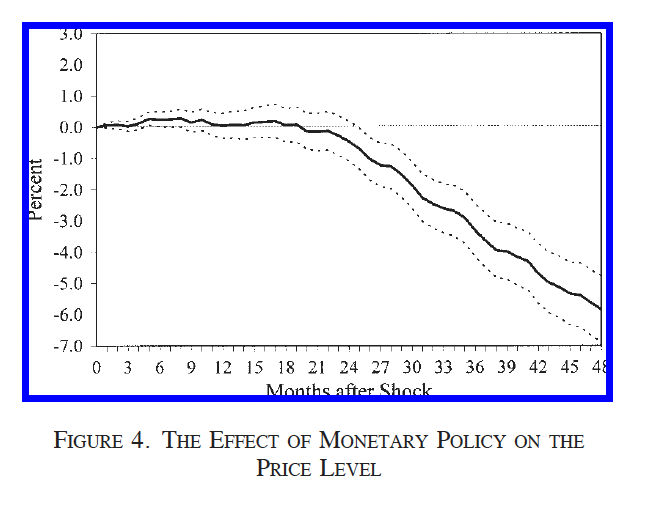
\includegraphics[width=0.4\textwidth]{FiguresTables/rr_p}
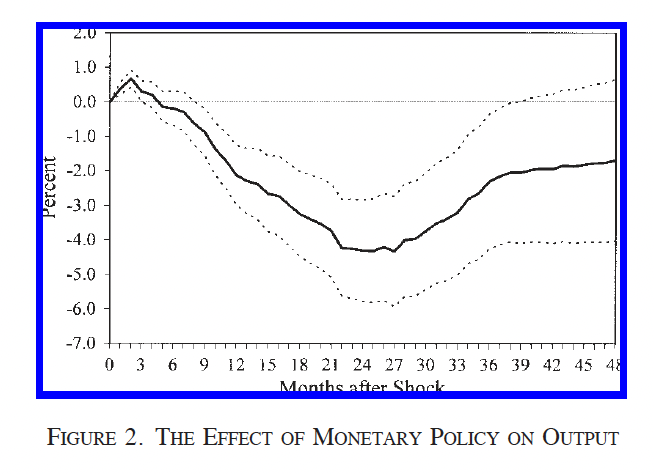
\includegraphics[width=0.4\textwidth]{FiguresTables/rr_y}
\caption{IRF of the Price Level and Output. Romer and Romer (2004)}
\end{figure}
\begin{itemize}
\item In the NK model, the CPI decreases on impact and keeps declining
\item In the data, the CPI seems to take a long time to react
\item Probably a failure of the model rather than one of causal inference.
\end{itemize}
\end{frame}

\begin{frame}{Estimating the NK model is hard}
\begin{align}
\hat{\pi_t} = {\color{blue}{\beta}}{\color{orange}{\mathbb{E}_t \hat{\pi}_{t+1}}} + {\color{blue}{\kappa}}(\hat{y}_t - {\color{orange}{\hat{y}^n_{t}}}) + {\color{orange}{\hat{\omega}_{t}}}
\end{align}
\begin{itemize}
\item Two parameters $\beta, \kappa$
\item Many unobservables $\mathbb{E}_t \hat{\pi}_{t+1}$, $\hat{y}^n_{t}$, $\hat{\omega}_{t}$
\item $\hat{y}_t$ may be dynamically correlated with those unobservables. Huge omitted variable bias problems
\item We will spend some time thinking about this
\end{itemize}
\end{frame}


\begin{frame}{Estimating the NK model is hard}
\begin{align}
\hat{y}_t &=-{\color{blue}{\sigma}}[\hat{i}_t-{\color{orange}{E_t\{\hat{\pi}_{t+1}\}}}]+{\color{orange}{E_t\{\hat{y}_{t+1}}\}}
\end{align}
\begin{itemize}
\item One parameter, $\sigma$. Actually two: the fact that future output enters with a coefficient of 1 is a testable implication.
\item Many unobservables $\mathbb{E}_t \hat{\pi}_{t+1}$, $\mathbb{E}_t \hat{y}_{t+1}$
\end{itemize}
\end{frame}

\end{document}


